\documentclass[12pt,a4paper]{article}
\usepackage[utf8]{inputenc}
\usepackage[T1]{fontenc}
\usepackage[french]{babel}
\usepackage{geometry}
\geometry{margin=2.5cm}
\usepackage[hidelinks]{hyperref}
\usepackage{graphicx}
\usepackage{listings}
\usepackage{xcolor}
\usepackage{booktabs}
\usepackage{longtable}
\usepackage{fancyhdr}
\usepackage{titlesec}
\usepackage{enumitem}
\usepackage{amssymb}
\usepackage{float}

\definecolor{codebg}{RGB}{245,245,245}
\definecolor{codeframe}{RGB}{200,200,200}
\lstset{
  backgroundcolor=\color{codebg},
  frame=single,
  rulecolor=\color{codeframe},
  basicstyle=\ttfamily\small,
  breaklines=true,
  showstringspaces=false,
  literate={é}{{\'e}}1 {è}{{\`e}}1 {ê}{{\^e}}1 {ë}{{\"e}}1
           {à}{{\`a}}1 {â}{{\^a}}1
           {ù}{{\`u}}1 {û}{{\^u}}1
           {î}{{\^i}}1 {ï}{{\"i}}1
           {ô}{{\^o}}1
           {ç}{{\c{c}}}1
           {É}{{\'E}}1 {È}{{\`E}}1
}

\pagestyle{fancy}
\fancyhf{}
\fancyhead[L]{DataShare --- Documentation Technique}
\fancyhead[R]{\thepage}
\fancyfoot[C]{OpenClassrooms --- Projet 4}

\title{
  \vspace{-2cm}
  \textbf{DataShare} \\
  \Large Documentation Technique Compl\`ete \\
  \vspace{0.5cm}
  \large Projet 4 --- OpenClassrooms, parcours Architecte logiciel \\
  \normalsize Mission « Pilotez le d\'eveloppement d'une solution informatique » \\
  \vspace{0.3cm}
  \normalsize D\'ep\^ot : \url{https://github.com/GadZouil/OC-P4-DataShare}
}
\author{Ethan Legros --- R\'ef\'erent technique senior, DataShare}
\date{Septembre 2026}

\begin{document}
\maketitle
\newpage
\tableofcontents
\newpage

%% ====================================================================
\section{Architecture de l'application}
%% ====================================================================

\subsection{Architecture g\'en\'erale}

DataShare adopte une architecture en \textbf{trois couches} inspir\'ee des principes Clean Architecture, o\`u chaque couche a une responsabilit\'e clairement d\'efinie :

\begin{itemize}[nosep]
  \item \textbf{API Layer} --- Contr\^oleurs ASP.NET Core (\texttt{AuthController}, \texttt{FilesController}, \texttt{PublicFilesController}) qui exposent les endpoints REST. Les DTOs (records et classes) sont d\'efinis directement dans les contr\^oleurs pour limiter la complexit\'e.
  \item \textbf{Service Layer} --- Logique m\'etier encapsul\'ee dans des services inject\'es : \texttt{IFileStorage} / \texttt{LocalFileStorage} (stockage fichiers), \texttt{ExpiredFilesCleanupService} (purge automatique), et ASP.NET Core Identity (\texttt{UserManager<AppUser>}) pour la gestion des utilisateurs.
  \item \textbf{Data Layer} --- Entity Framework Core 9 avec le \texttt{DataShareDbContext} (h\'eritant de \texttt{IdentityDbContext}) communiquant avec PostgreSQL 16 via le provider Npgsql.
\end{itemize}

Le \textbf{frontend} est une Single Page Application Vue~3 (Composition API + TypeScript) servie par Vite, qui consomme l'API REST via Axios.

\begin{figure}[H]
  \centering
  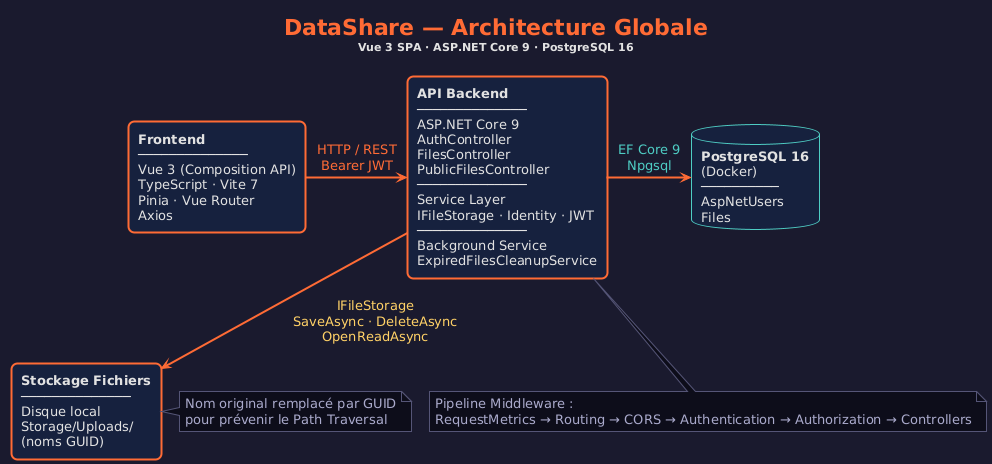
\includegraphics[width=\textwidth,keepaspectratio]{diagrams/architecture_globale.drawio.png}
  \caption{Architecture globale de DataShare --- Vue 3 SPA, API ASP.NET Core 9, PostgreSQL 16 et stockage fichiers}
\end{figure}

\subsection{Structure du projet}

\begin{lstlisting}[title={Arborescence du projet}]
OC-P4-DataShare/
  backend/
    DataShare.Api/
      Controllers/        # AuthController, FilesController, PublicFilesController
      Data/               # DataShareDbContext
      Middleware/         # RequestMetricsMiddleware (logs structures par requete)
      Migrations/         # 4 migrations EF Core
      Models/             # AppUser, FileItem
      Services/           # IFileStorage, LocalFileStorage, ExpiredFilesCleanupService
      Program.cs          # Point d'entree, DI, middleware pipeline
      appsettings.json    # Configuration (connexion DB, JWT, CORS, logs)
      DataShare.Api.csproj
    DataShare.Api.Tests/
      Helpers/            # CustomWebApplicationFactory, FakeFileStorage, TestAuthHandler
      IntegrationTests/   # 10 fichiers, 39 tests d'integration
      UnitTests/          # ExpiredFilesCleanupServiceTests (2 tests)
    DataShare.sln
    Dockerfile            # Build .NET 9 multi-stage
  frontend/
    datashare-front/
      src/
        api/              # auth.ts, files.ts (clients HTTP)
        layouts/          # PublicLayout.vue
        router/           # index.ts (5 routes + garde d'authentification)
        services/         # api.ts (instance Axios : JWT, gestion du 401)
        stores/           # auth.ts (Pinia)
        styles/           # datashare.css (charte Figma)
        views/            # 5 vues : Login, Register, Upload, Me, Download
        App.vue, main.ts
      vite.config.ts
      package.json
    cypress/
      e2e/                # 5 fichiers de tests E2E
      support/            # commands.ts, e2e.ts
    Dockerfile            # Node 20 + Nginx
  docs/
    diagrams/             # architecture, MCD, flux (PlantUML + PNG, draw.io)
    API_REFERENCE.md      # Documentation API complete
    openapi.yaml          # Contrat d'interface OpenAPI 3
    soutenance/           # Support de presentation, script oral, scenario de demo
  perf/                   # Scripts k6 (upload, login)
  scripts/                # deploy.ps1/.sh, db-backup.ps1, db-restore.ps1, verify.ps1
  docker-compose.yml      # 3 services : db, api, frontend (secrets lus dans .env)
  .env.example
  README.md, SECURITY.md, TESTING.md, PERF.md, MAINTENANCE.md, AI_USAGE.md
\end{lstlisting}

\subsection{Patterns utilis\'es}

\begin{description}[style=nextline]
  \item[Dependency Injection (DI)]
    Le conteneur IoC natif d'ASP.NET Core est utilis\'e intensivement. Dans \texttt{Program.cs}, les services sont enregistr\'es via \texttt{AddSingleton<IFileStorage, LocalFileStorage>()} et \texttt{AddIdentityCore<AppUser>()}. Les contr\^oleurs re\c{c}oivent leurs d\'ependances par injection de constructeur (\texttt{DataShareDbContext}, \texttt{IFileStorage}, \texttt{UserManager<AppUser>}).

  \item[Interface Segregation (IFileStorage)]
    Le stockage de fichiers est abstrait derri\`ere l'interface \texttt{IFileStorage} d\'efinissant trois op\'erations : \texttt{SaveAsync}, \texttt{DeleteAsync}, \texttt{OpenReadAsync}. L'impl\'ementation \texttt{LocalFileStorage} stocke les fichiers sur le syst\`eme de fichiers local dans \texttt{Storage/Uploads/}. Cette abstraction permet de remplacer le stockage par un provider cloud (Azure Blob, S3) sans modifier les contr\^oleurs.

  \item[DTOs (Data Transfer Objects)]
    Les records C\# (\texttt{MyFileDto}, \texttt{AuthResponse}, \texttt{RegisterRequest}, \texttt{LoginRequest}) et classes (\texttt{UploadRequest}, \texttt{DownloadRequest}) sont d\'efinis dans les contr\^oleurs pour d\'ecoupler le mod\`ele de domaine des r\'eponses API. Les propri\'et\'es calcul\'ees (\texttt{IsExpired}, \texttt{IsPasswordProtected}) du mod\`ele ne sont pas expos\'ees directement.

  \item[Background Service]
    \texttt{ExpiredFilesCleanupService} h\'erite de \texttt{BackgroundService} et s'ex\'ecute automatiquement au d\'emarrage puis toutes les 24 heures via un \texttt{PeriodicTimer}. Il purge les fichiers expir\'es (stockage disque + entr\'ees en base) en utilisant un scope de DI d\'edi\'e (\texttt{IServiceScopeFactory}).

  \item[Middleware Pipeline]
    Le pipeline HTTP est configur\'e dans \texttt{Program.cs} avec l'ordre : \texttt{UseRequestMetrics} (journalisation structur\'ee de chaque requ\^ete) $\rightarrow$ \texttt{UseRouting} $\rightarrow$ \texttt{UseCors} $\rightarrow$ \texttt{UseAuthentication} $\rightarrow$ \texttt{UseAuthorization} $\rightarrow$ \texttt{MapControllers}. Le middleware de m\'etriques est plac\'e en t\^ete pour mesurer le temps total, authentification comprise.
\end{description}

\begin{figure}[H]
  \centering
  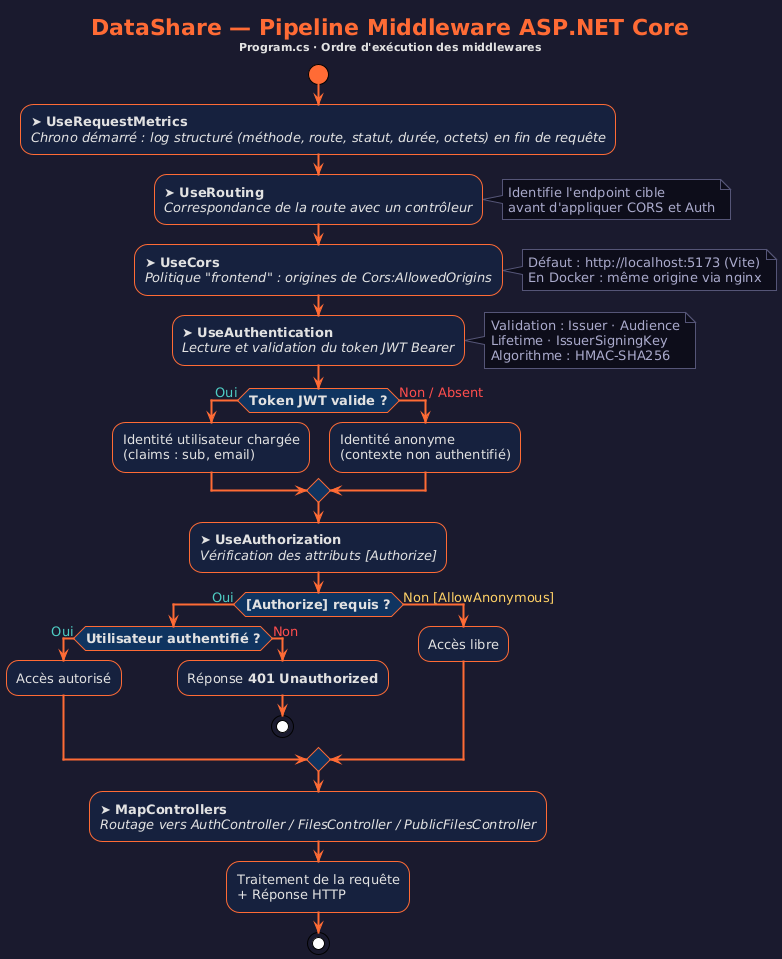
\includegraphics[width=0.72\textwidth,keepaspectratio]{diagrams/pipeline_middleware.drawio.png}
  \caption{Pipeline middleware ASP.NET Core --- ordre d'ex\'ecution et bifurcations d'autorisation}
\end{figure}

%% ====================================================================
\section{Choix technologiques justifi\'es}
%% ====================================================================

Les versions ci-dessous sont extraites directement des fichiers \texttt{DataShare.Api.csproj} et \texttt{package.json} du projet.

\subsection{Backend}

\begin{longtable}{p{5.5cm} p{2cm} p{7cm}}
\toprule
\textbf{Technologie} & \textbf{Version} & \textbf{Justification} \\
\midrule
\endhead
ASP.NET Core & 9.0 & Framework web performant, multiplateforme, support natif de l'injection de d\'ependances et du middleware pipeline. \\
Entity Framework Core & 9.0.1 & ORM mature pour .NET, migrations automatiques, protection contre les injections SQL par param\'etrisation des requ\^etes. \\
Npgsql (EF Core PostgreSQL) & 9.0.1 & Provider EF Core pour PostgreSQL, support natif des types PostgreSQL (\texttt{text[]}) pour les tags. \\
PostgreSQL & 16 & Base relationnelle open source robuste, support des tableaux natifs (\texttt{text[]}), excellentes performances en lecture/\'ecriture. \\
ASP.NET Core Identity & 9.0.1 & Gestion compl\`ete des utilisateurs (hachage PBKDF2, validation email, contraintes mot de passe) sans code custom. \\
JWT Bearer Authentication & 9.0.1 & Authentification stateless adapt\'ee aux SPA, tokens sign\'es HMAC-SHA256, dur\'ee de vie configurable (8h). \\
System.IdentityModel.Tokens.Jwt & 8.15.0 & Cr\'eation et validation des tokens JWT c\^ot\'e serveur. \\
Swashbuckle (Swagger) & 10.1.0 & G\'en\'eration automatique de la documentation OpenAPI, UI interactive en d\'eveloppement. \\
\bottomrule
\end{longtable}

\subsection{Tests Backend}

\begin{longtable}{p{5.5cm} p{2cm} p{7cm}}
\toprule
\textbf{Technologie} & \textbf{Version} & \textbf{Justification} \\
\midrule
\endhead
xUnit & 2.9.2 & Framework de tests standard pour .NET, support des th\'eories et faits, parall\'elisation native. \\
FluentAssertions & 6.12.1 & Assertions lisibles en langage naturel (\texttt{result.Should().Be200Ok()}). \\
Moq & 4.20.72 & Cr\'eation de mocks pour isoler les unit\'es de code (services, stockage). \\
Microsoft.AspNetCore.Mvc.Testing & 9.0.0 & \texttt{WebApplicationFactory} pour les tests d'int\'egration HTTP sans serveur r\'eel. \\
EF Core InMemory & 9.0.0 & Base de donn\'ees en m\'emoire pour les tests d'int\'egration, remplacement transparent de PostgreSQL. \\
Coverlet & 6.0.4 & Collecte de couverture de code au format Cobertura, int\'egr\'e \`a \texttt{dotnet test}. \\
ReportGenerator & 5.5.1 & G\'en\'eration de rapports HTML de couverture depuis les fichiers Cobertura. \\
\bottomrule
\end{longtable}

\subsection{Frontend}

\begin{longtable}{p{5.5cm} p{2cm} p{7cm}}
\toprule
\textbf{Technologie} & \textbf{Version} & \textbf{Justification} \\
\midrule
\endhead
Vue 3 & 3.5.26 & Framework r\'eactif avec Composition API, \'ecosyst\`eme riche, courbe d'apprentissage accessible. \\
TypeScript & 5.9.3 & Typage statique pour la fiabilit\'e du code frontend, autocompl\'etion IDE am\'elior\'ee. \\
Vite & 7.3.0 & Bundler ultra-rapide (ESBuild + Rollup), HMR instantan\'e, tree-shaking en production. \\
Pinia & 3.0.4 & Store centralis\'e pour Vue 3, API simple et type-safe, remplacement officiel de Vuex. \\
Vue Router & 4.6.4 & Routeur officiel, lazy-loading des composants, mode \texttt{history} HTML5. \\
Axios & 1.13.2 & Client HTTP avec intercepteurs pour l'injection automatique du token JWT. \\
Cypress & 15.10.0 & Tests E2E fiables, interface graphique interactive, assertions cha\^in\'ees, screenshots automatiques. \\
\bottomrule
\end{longtable}

\subsection{Infrastructure}

\begin{longtable}{p{5.5cm} p{2cm} p{7cm}}
\toprule
\textbf{Technologie} & \textbf{Version} & \textbf{Justification} \\
\midrule
\endhead
Docker & -- & Conteneurisation de tous les services pour un d\'eploiement reproductible. \\
Docker Compose & -- & Orchestration locale des 3 services (PostgreSQL, API, Frontend) en une commande. \\
Nginx & alpine & Serveur de fichiers statiques l\'eger pour le frontend en production. \\
Node.js & 20+ & Runtime pour le build frontend (Vite) et les tests Cypress. \\
\bottomrule
\end{longtable}

%% ====================================================================
\section{Mod\`ele de donn\'ees}
%% ====================================================================

Le mod\`ele de donn\'ees repose sur deux entit\'es m\'etier et les tables syst\`eme g\'en\'er\'ees par ASP.NET Core Identity.

\subsection{Entit\'e AppUser}

\texttt{AppUser} h\'erite de \texttt{IdentityUser<Guid>} sans propri\'et\'es suppl\'ementaires. Les propri\'et\'es h\'erit\'ees sont g\'er\'ees par Identity :

\begin{longtable}{p{4.5cm} p{3.5cm} p{6.5cm}}
\toprule
\textbf{Propri\'et\'e} & \textbf{Type C\#} & \textbf{Description} \\
\midrule
\endhead
Id & \texttt{Guid} & Cl\'e primaire (GUID) \\
UserName & \texttt{string} & Nom d'utilisateur (= email) \\
Email & \texttt{string} & Adresse email (unique) \\
PasswordHash & \texttt{string} & Hash PBKDF2 du mot de passe \\
SecurityStamp & \texttt{string} & Jeton de s\'ecurit\'e (invalidation sessions) \\
ConcurrencyStamp & \texttt{string} & Contr\^ole de concurrence optimiste \\
\bottomrule
\end{longtable}

\subsection{Entit\'e FileItem}

\begin{longtable}{p{4.5cm} p{3.5cm} p{6.5cm}}
\toprule
\textbf{Propri\'et\'e} & \textbf{Type C\#} & \textbf{Description} \\
\midrule
\endhead
Id & \texttt{Guid} & PK, g\'en\'er\'e par \texttt{Guid.NewGuid()} \\
OwnerId & \texttt{Guid?} & FK nullable vers \texttt{AppUser.Id} \\
Owner & \texttt{AppUser?} & Navigation vers le propri\'etaire \\
OriginalFileName & \texttt{string} & Nom original du fichier (\texttt{[MaxLength(255)]}) \\
StoredFileName & \texttt{string} & Nom sur disque (GUID + extension) \\
ContentType & \texttt{string?} & Type MIME (\texttt{[MaxLength(255)]}) \\
SizeBytes & \texttt{long} & Taille en octets \\
Token & \texttt{string} & Token de partage unique (\texttt{[MaxLength(128)]}, index unique) \\
CreatedAt & \texttt{DateTimeOffset} & Date de cr\'eation \\
ExpiresAt & \texttt{DateTimeOffset} & Date d'expiration \\
PasswordHash & \texttt{string?} & Hash du mot de passe de protection \\
Tags & \texttt{string[]} & Tags (PostgreSQL \texttt{text[]}) \\
IsExpired & \texttt{bool} & Propri\'et\'e calcul\'ee (non mapp\'ee) \\
IsPasswordProtected & \texttt{bool} & Propri\'et\'e calcul\'ee (non mapp\'ee) \\
\bottomrule
\end{longtable}

\subsection{Relations}

\begin{figure}[H]
  \centering
  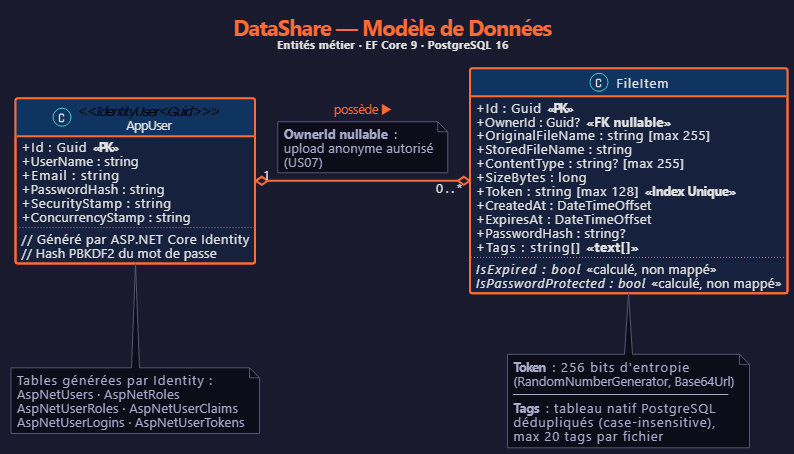
\includegraphics[width=\textwidth,keepaspectratio]{diagrams/modele_donnees.drawio.png}
  \caption{Mod\`ele de donn\'ees --- entit\'es \texttt{AppUser} et \texttt{FileItem}, relation 1:N avec \texttt{OwnerId} nullable}
\end{figure}

\begin{itemize}[nosep]
  \item \textbf{AppUser (1) $\rightarrow$ (N) FileItem} : un utilisateur peut poss\'eder plusieurs fichiers. La relation est optionnelle (\texttt{OwnerId} nullable) pour permettre les uploads anonymes (US07).
  \item Pas de table de jointure : les tags sont stock\'es comme tableau PostgreSQL natif (\texttt{text[]}) directement dans la table \texttt{Files}.
  \item L'index unique sur \texttt{Token} garantit l'unicit\'e des liens de partage.
\end{itemize}

\subsection{Configuration Fluent API}

La configuration du mod\`ele est d\'efinie dans \texttt{DataShareDbContext.OnModelCreating} :

\begin{lstlisting}
builder.Entity<FileItem>(e =>
{
    e.HasIndex(x => x.Token).IsUnique();
    e.Property(x => x.Tags).HasColumnType("text[]");
});
\end{lstlisting}

\subsection{Historique des migrations}

\begin{longtable}{p{2cm} p{5cm} p{7.5cm}}
\toprule
\textbf{Date} & \textbf{Migration} & \textbf{Description} \\
\midrule
\endhead
05/01/2026 & InitialAuth & Tables Identity (AspNetUsers, AspNetRoles, etc.) \\
06/01/2026 & AddFiles & Table \texttt{Files} avec FK vers AspNetUsers \\
16/01/2026 & MakeFileOwnerNullable & Pr\'eparation pour OwnerId nullable \\
19/01/2026 & MakeOwnerIdNullable & OwnerId rendu nullable (uploads anonymes) \\
\bottomrule
\end{longtable}

%% ====================================================================
\section{Documentation d'API}
%% ====================================================================

L'API REST est document\'ee automatiquement via Swagger (Swashbuckle) accessible en environnement de d\'eveloppement (\texttt{dotnet run}) sur \texttt{http://localhost:5180/swagger} ; le contrat de r\'ef\'erence est \texttt{docs/openapi.yaml} (OpenAPI 3, valid\'e), doubl\'e de \texttt{docs/API\_REFERENCE.md}. Le token JWT est obtenu via \texttt{POST /api/auth/register} ou \texttt{POST /api/auth/login} et expire apr\`es \textbf{8 heures}.

\subsection{Auth --- \texttt{/api/auth}}

\begin{longtable}{p{1.2cm} p{3.5cm} p{3cm} p{1cm} p{5cm}}
\toprule
\textbf{M\'eth.} & \textbf{Route} & \textbf{Description} & \textbf{Auth} & \textbf{Codes retour} \\
\midrule
\endhead
POST & \texttt{/api/auth/register} & Inscription & Non & 200 OK, 400 Bad Request \\
POST & \texttt{/api/auth/login} & Connexion & Non & 200 OK, 401 Unauthorized \\
\bottomrule
\end{longtable}

\textbf{Corps de requ\^ete (register \& login) :}
\begin{lstlisting}
{
  "email": "alice@example.com",
  "password": "MonMotDePasse1!"
}
\end{lstlisting}

\textbf{R\'eponse succ\`es (200 OK) :}
\begin{lstlisting}
{
  "token": "eyJhbGciOiJIUzI1NiIsInR5cCI6IkpXVCJ9..."
}
\end{lstlisting}

\subsection{Files (authentifi\'e) --- \texttt{/api/files}}

\begin{longtable}{p{1.2cm} p{3.3cm} p{3.5cm} p{1cm} p{4.5cm}}
\toprule
\textbf{M\'eth.} & \textbf{Route} & \textbf{Description} & \textbf{Auth} & \textbf{Codes retour} \\
\midrule
\endhead
POST & \texttt{/api/files} & Upload fichier & Oui & 201, 400, 401 \\
GET & \texttt{/api/files} & Lister ses fichiers & Oui & 200, 401 \\
GET & \texttt{/api/files/me} & Lister (variante) & Oui & 200, 401 \\
GET & \texttt{/api/files/\{id\}} & D\'etail d'un fichier & Oui & 200, 401, 404 \\
DELETE & \texttt{/api/files/\{id\}} & Supprimer un fichier & Oui & 204, 401, 404 \\
\bottomrule
\end{longtable}

\textbf{Upload --- Corps multipart/form-data :}

\begin{longtable}{p{3.5cm} p{2cm} p{1.5cm} p{7cm}}
\toprule
\textbf{Champ} & \textbf{Type} & \textbf{Requis} & \textbf{Description} \\
\midrule
\endhead
\texttt{file} & binary & Oui & Fichier (max 1 Go) \\
\texttt{expiresInDays} & integer & Non & Dur\'ee 1--7 jours (d\'efaut : 7) \\
\texttt{password} & string & Non & Mot de passe (min 6 caract\`eres) \\
\texttt{tags} & string[] & Non & Tags (max 20, d\'edupliqu\'es) \\
\bottomrule
\end{longtable}

\textbf{R\'eponse upload (201 Created) :}
\begin{lstlisting}
{
  "id": "3fa85f64-5717-4562-b3fc-2c963f66afa6",
  "originalFileName": "rapport.pdf",
  "sizeBytes": 204800,
  "contentType": "application/pdf",
  "createdAt": "2026-03-10T14:00:00Z",
  "expiresAt": "2026-03-17T14:00:00Z",
  "token": "abc123XYZ_urlsafe_base64",
  "passwordRequired": false,
  "tags": ["projet", "2026"]
}
\end{lstlisting}

\textbf{R\'eponse listing (200 OK) :}
\begin{lstlisting}
[
  {
    "id": "3fa85f64-5717-4562-b3fc-2c963f66afa6",
    "originalFileName": "rapport.pdf",
    "sizeBytes": 204800,
    "contentType": "application/pdf",
    "createdAt": "2026-03-10T14:00:00Z",
    "expiresAt": "2026-03-17T14:00:00Z",
    "token": "abc123XYZ_urlsafe_base64",
    "passwordRequired": false,
    "tags": ["projet"],
    "isExpired": false
  }
]
\end{lstlisting}

\textbf{Param\`etre de filtre :} \texttt{?status=all|active|expired} (d\'efaut : \texttt{all}).

\textbf{Extensions interdites :} \texttt{.exe}, \texttt{.bat}, \texttt{.cmd}, \texttt{.com}, \texttt{.msi}, \texttt{.scr}, \texttt{.ps1}.

\begin{figure}[H]
  \centering
  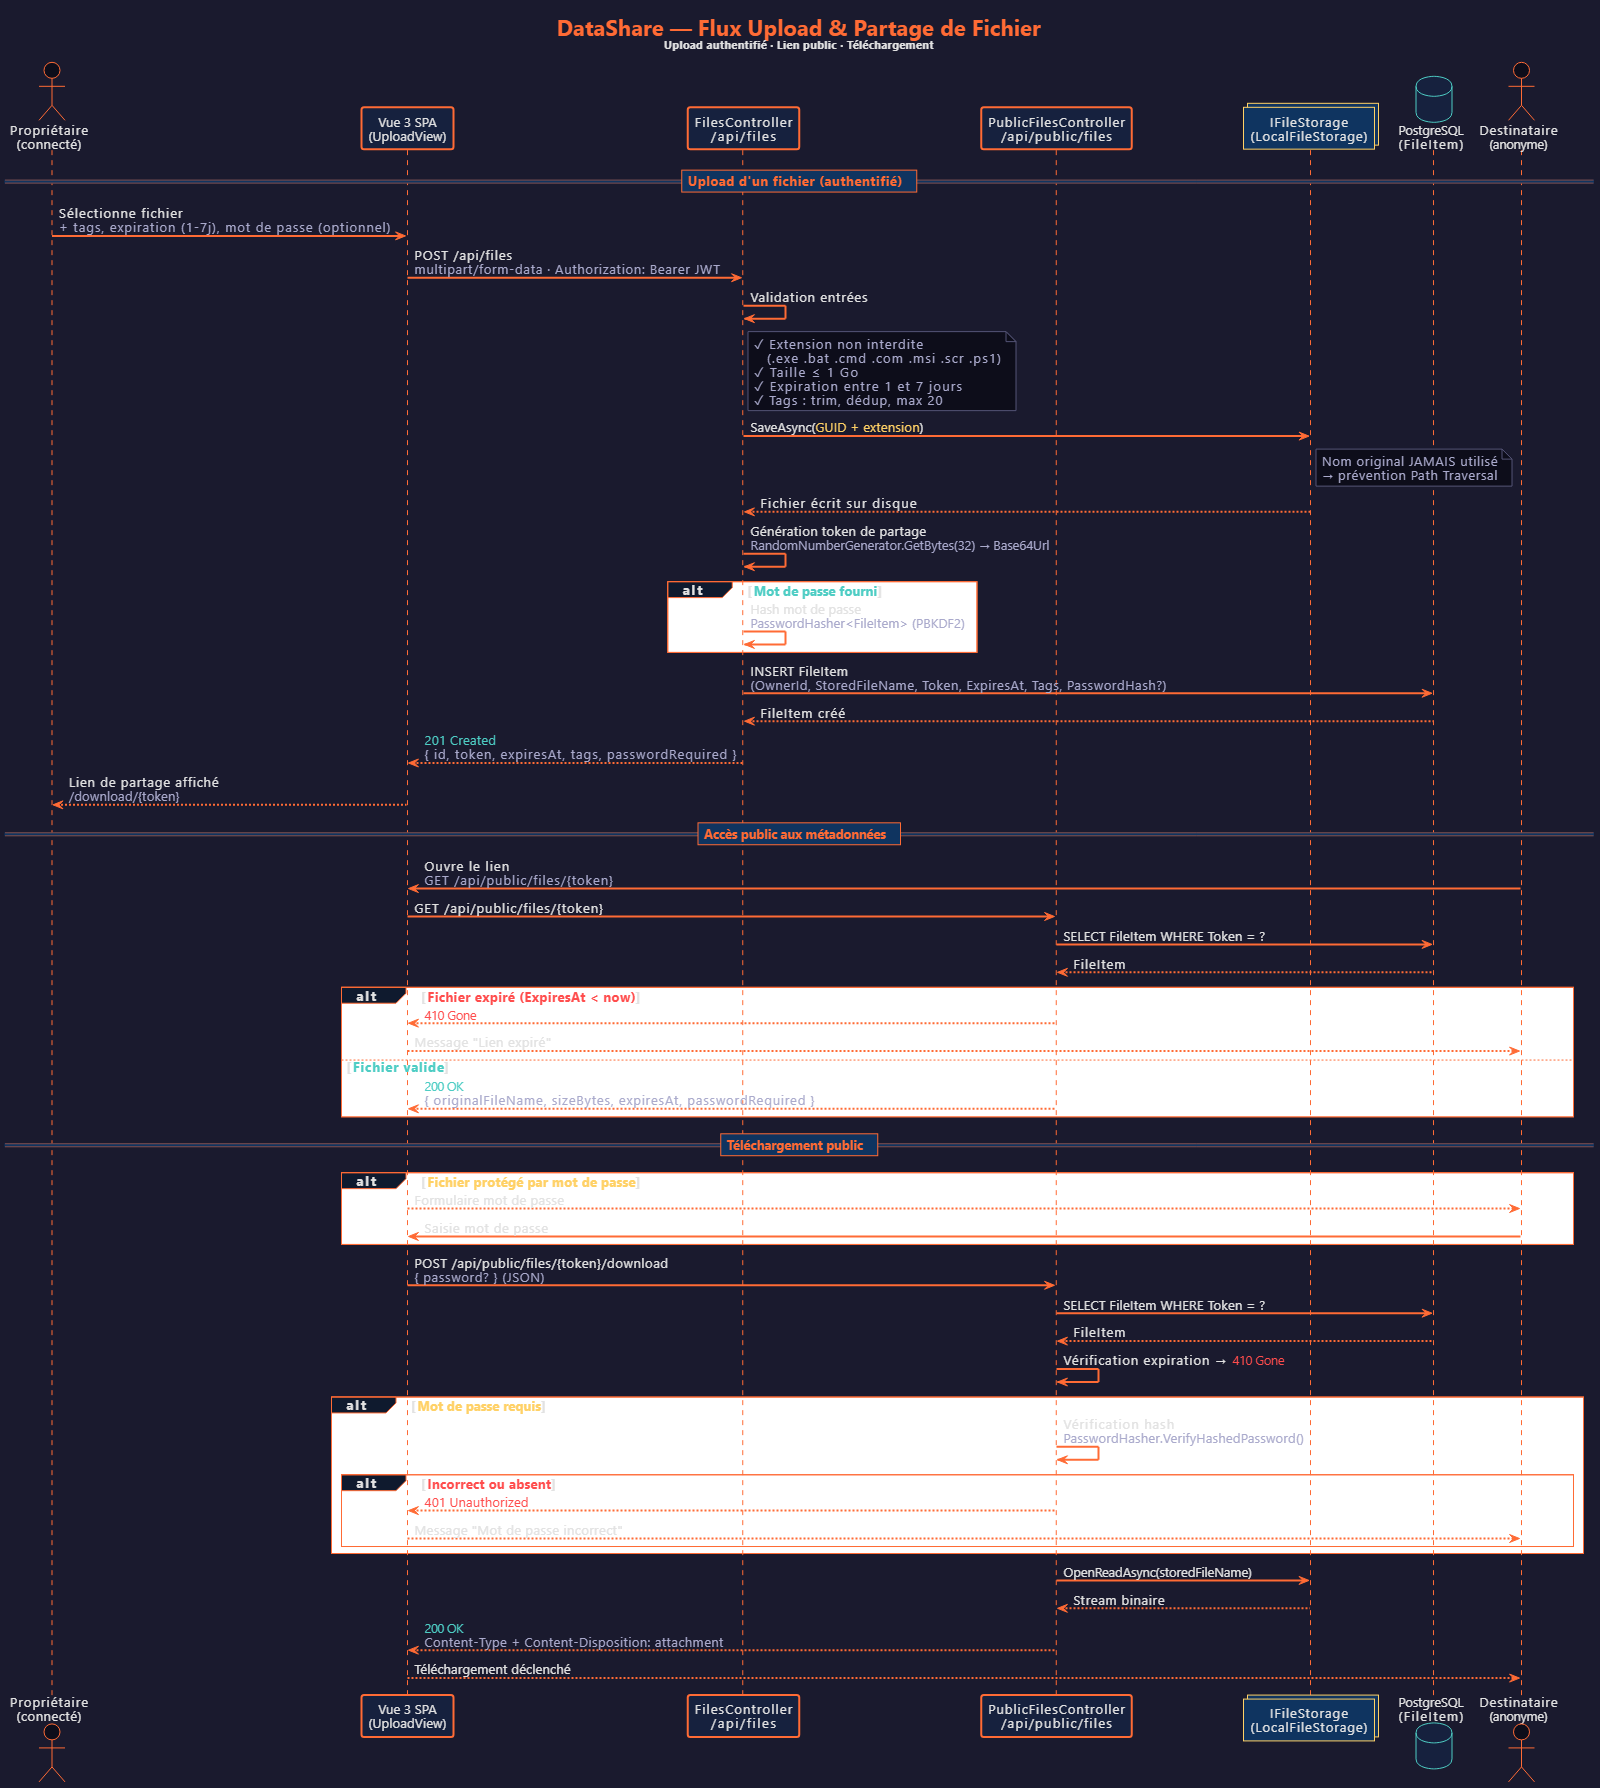
\includegraphics[width=\textwidth,height=0.88\textheight,keepaspectratio]{diagrams/flux_upload_partage.drawio.png}
  \caption{Flux upload et partage --- cycle complet de l'upload authentifi\'e au t\'el\'echargement public}
\end{figure}

\subsection{Liens publics --- \texttt{/api/public/files}}

\begin{longtable}{p{1.2cm} p{4.8cm} p{3cm} p{1cm} p{3.5cm}}
\toprule
\textbf{M\'eth.} & \textbf{Route} & \textbf{Description} & \textbf{Auth} & \textbf{Codes retour} \\
\midrule
\endhead
POST & \texttt{/api/public/files} & Upload anonyme & Non* & 201, 400, 403 \\
GET & \texttt{/api/public/files/\{token\}} & M\'etadonn\'ees & Non & 200, 404, 410 \\
POST & \texttt{/api/public/files/\{token\}/download} & T\'el\'echargement & Non & 200, 401, 404, 410 \\
\bottomrule
\end{longtable}

\small{* L'upload anonyme est interdit si l'utilisateur est d\'ej\`a authentifi\'e (403 Forbidden).}

\normalsize

\textbf{T\'el\'echargement --- Corps JSON (optionnel si non prot\'eg\'e) :}
\begin{lstlisting}
{
  "password": "monMotDePasse"
}
\end{lstlisting}

\textbf{R\'eponse succ\`es :} Stream binaire avec headers \texttt{Content-Type} et \texttt{Content-Disposition: attachment}.

\textbf{Codes sp\'ecifiques :}
\begin{itemize}[nosep]
  \item \textbf{410 Gone} : le lien est expir\'e.
  \item \textbf{401 Unauthorized} : mot de passe requis mais absent ou incorrect.
\end{itemize}

%% ====================================================================
\section{S\'ecurit\'e et gestion des acc\`es}
%% ====================================================================

La s\'ecurit\'e de DataShare repose sur une approche de d\'efense en profondeur (Defense in Depth), o\`u chaque couche de l'application impl\'emente ses propres m\'ecanismes de protection.

\subsection{Authentification JWT}

L'authentification utilise exclusivement des JSON Web Tokens (JWT), rendant le serveur stateless (aucune session c\^ot\'e serveur). La configuration est d\'efinie dans \texttt{Program.cs} :

\begin{itemize}[nosep]
  \item \textbf{Algorithme :} HMAC-SHA256 (\texttt{SecurityAlgorithms.HmacSha256})
  \item \textbf{Dur\'ee de vie :} 8 heures (\texttt{DateTime.UtcNow.AddHours(8)})
  \item \textbf{Validation :} Issuer, Audience, Lifetime et IssuerSigningKey sont tous valid\'es
  \item \textbf{Claims :} \texttt{sub} (ID utilisateur) et \texttt{email}
  \item \textbf{Cl\'e :} lue dans la configuration (\texttt{Jwt:Key}, variable d'environnement \texttt{Jwt\_\_Key} ou user-secrets). L'API \textbf{refuse de d\'emarrer} si la cl\'e est absente ou fait moins de 32 caract\`eres : aucune cl\'e de repli n'est cod\'ee en dur.
  \item \textbf{\'Echec de connexion :} r\'eponse \texttt{401} identique que l'email soit inconnu ou le mot de passe faux (pas d'\'enum\'eration de comptes).
\end{itemize}

Les contr\^oleurs prot\'eg\'es utilisent l'attribut \texttt{[Authorize]} au niveau de la classe (\texttt{FilesController}). L'identit\'e de l'utilisateur est extraite du claim \texttt{NameIdentifier} pour filtrer l'acc\`es aux fichiers.

\begin{figure}[H]
  \centering
  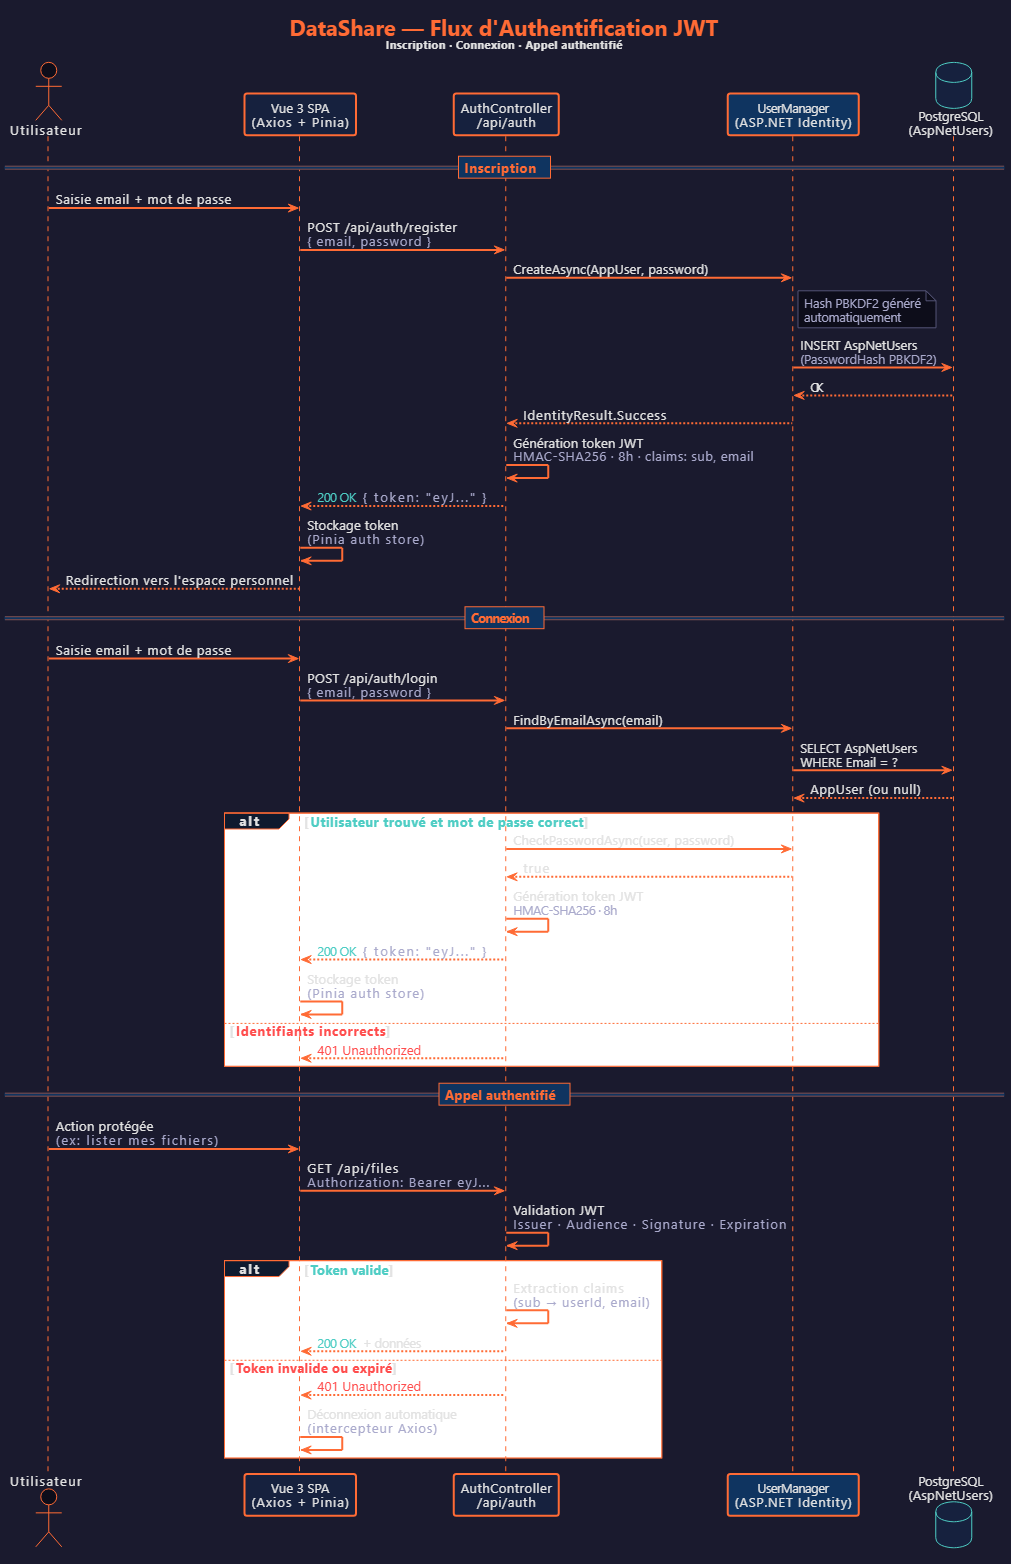
\includegraphics[width=\textwidth,height=0.88\textheight,keepaspectratio]{diagrams/flux_authentification.drawio.png}
  \caption{Flux d'authentification JWT --- inscription, connexion et appel authentifi\'e}
\end{figure}

\subsection{Hachage des mots de passe}

\begin{itemize}[nosep]
  \item \textbf{Mots de passe utilisateur :} hach\'es par ASP.NET Core Identity via \textbf{PBKDF2} (impl\'ementation standard \texttt{PasswordHasher<TUser>}), rendant les attaques par Rainbow Table impraticables.
  \item \textbf{Mots de passe de fichiers :} hach\'es \'egalement via \texttt{PasswordHasher<FileItem>} avec le m\^eme algorithme PBKDF2.
  \item \textbf{Contraintes :} minimum 8 caract\`eres pour les comptes utilisateur, minimum 6 caract\`eres pour la protection des fichiers.
\end{itemize}

\subsection{Validation des entr\'ees}

\begin{itemize}[nosep]
  \item \textbf{Taille des fichiers :} limit\'ee \`a 1 Go via \texttt{[RequestSizeLimit]} et \texttt{FormOptions.MultipartBodyLengthLimit}.
  \item \textbf{Extensions interdites :} les ex\'ecutables (\texttt{.exe}, \texttt{.bat}, \texttt{.cmd}, \texttt{.com}, \texttt{.msi}, \texttt{.scr}, \texttt{.ps1}) sont rejet\'es au niveau du contr\^oleur.
  \item \textbf{Dur\'ee d'expiration :} valid\'ee entre 1 et 7 jours.
  \item \textbf{Tags :} nettoy\'es (trim), d\'edupliqu\'es (case-insensitive), limit\'es \`a 20 par fichier.
  \item \textbf{Data Annotations :} \texttt{[Required]}, \texttt{[MaxLength(255)]} et \texttt{[MaxLength(128)]} sur les propri\'et\'es du mod\`ele \texttt{FileItem}.
\end{itemize}

\subsection{Protection des fichiers}

\begin{itemize}[nosep]
  \item \textbf{Sanitization des noms :} aucun fichier n'est stock\'e avec son nom d'origine. Il est remplac\'e par un GUID al\'eatoire (\texttt{Guid.NewGuid()}) pour emp\^echer les attaques de type Path Traversal.
  \item \textbf{Isolation logique :} l'identit\'e vient uniquement du token (\texttt{User.FindFirstValue(ClaimTypes.NameIdentifier)}) et chaque requ\^ete priv\'ee filtre sur \texttt{OwnerId == userId} ; un fichier d'un autre utilisateur r\'epond \texttt{404} (et non \texttt{403}) pour ne pas r\'ev\'eler son existence. Ces r\`egles sont v\'erifi\'ees par les tests d'int\'egration \texttt{SecurityTests} (lecture et suppression crois\'ees, \texttt{/files/me} isol\'e par utilisateur, endpoints priv\'es sans token, m\'etadonn\'ees publiques sans \texttt{ownerId} ni \texttt{token}).
  \item \textbf{Token de partage :} g\'en\'er\'e cryptographiquement via \texttt{RandomNumberGenerator.GetBytes(32)} encod\'e en Base64Url (256 bits d'entropie).
\end{itemize}

\subsection{Anti-injection SQL}

L'utilisation stricte d'Entity Framework Core (ORM) param\`etre toutes les requ\^etes, neutralisant les injections SQL classiques. Aucune requ\^ete SQL brute n'est utilis\'ee dans le projet.

\subsection{CORS}

La politique CORS nomm\'ee \texttt{"frontend"} (\texttt{Program.cs}) n'accepte que les origines list\'ees dans \texttt{Cors:AllowedOrigins} (par d\'efaut \texttt{http://localhost:5173}, le serveur de d\'eveloppement Vite ; surchargeable par \texttt{CORS\_ALLOWED\_ORIGINS} dans \texttt{.env}). L'en-t\^ete \texttt{Content-Disposition} est expos\'e pour que le front lise le nom du fichier t\'el\'echarg\'e. En Docker, nginx sert le front et proxifie \texttt{/api} en m\^eme origine : CORS n'entre pas en jeu.

\subsection{Transport et journalisation}

Le prototype est servi en HTTP sur \texttt{localhost} ; HTTPS n'est pas activ\'e dans le code. En production, la terminaison TLS est pr\'evue sur le reverse proxy nginx (certificat Let's Encrypt), pratique standard pour une API conteneuris\'ee. Chaque requ\^ete produit une ligne de log structur\'ee (m\'ethode, route, statut, dur\'ee, volume) et les refus de mot de passe sur un fichier prot\'eg\'e sont trac\'es en \texttt{Warning} ; aucun mot de passe ni token complet n'est journalis\'e (voir section~\ref{sec:logs}).

\subsection{Gestion des secrets}

\begin{itemize}[nosep]
  \item \textbf{D\'eveloppement :} User Secrets .NET (\texttt{secrets.json}). Les cl\'es JWT et cha\^ines de connexion ne sont pas commit\'ees dans Git. Le fichier \texttt{.env.example} fournit un template.
  \item \textbf{Production :} les secrets sont inject\'es via des variables d'environnement (Docker Compose ou CI/CD).
\end{itemize}

\subsection{Am\'eliorations futures}

\begin{itemize}[nosep]
  \item HTTPS / HSTS : terminaison TLS sur nginx puis \texttt{UseHttpsRedirection()} et \texttt{UseHsts()} derri\`ere \texttt{ForwardedHeaders}.
  \item Rate Limiting (\texttt{AddRateLimiter}, natif .NET) sur \texttt{/auth/login} et le t\'el\'echargement prot\'eg\'e (pr\'evention brute force).
  \item Refresh Tokens pour r\'eduire la dur\'ee de vie des access tokens (8~h aujourd'hui).
  \item Liste blanche d'extensions et v\'erification du type r\'eel (signature) en compl\'ement de la liste noire actuelle.
  \item En-t\^etes de s\'ecurit\'e (CSP, \texttt{X-Content-Type-Options}) c\^ot\'e nginx.
  \item Scan antivirus des uploads (ClamAV via nClam) et chiffrement au repos (impl\'ementation \texttt{IFileStorage} d\'edi\'ee).
\end{itemize}

%% ====================================================================
\section{Qualit\'e, tests et maintenance}
%% ====================================================================

\subsection{Strat\'egie de tests}

L'approche qualit\'e repose sur la \textbf{pyramide des tests}, privil\'egiant une base solide de tests unitaires et d'int\'egration pour garantir la robustesse du backend .NET.

\begin{description}[style=nextline]
  \item[Tests unitaires]
    Validation de la logique m\'etier isol\'ee (services) via des mocks (Moq). Exemple : \texttt{ExpiredFilesCleanupServiceTests} valide la purge des fichiers expir\'es sans d\'ependance au syst\`eme de fichiers r\'eel gr\^ace \`a un mock Moq de \texttt{IFileStorage}.

  \item[Tests d'int\'egration]
    Validation des endpoints API dans un environnement complet via \texttt{WebApplicationFactory} et une base de donn\'ees en m\'emoire (EF Core InMemory) ; le stockage passe par le vrai \texttt{LocalFileStorage} dans un dossier ignor\'e par Git. Authentification simul\'ee par un \texttt{TestAuthHandler} personnalis\'e, qui accepte un en-t\^ete \texttt{X-Test-UserId} pour incarner un second utilisateur. 10 fichiers, \textbf{39 tests}, couvrent : authentification (dont email dupliqu\'e, mot de passe court, email inconnu), upload, listing (\texttt{/files} et \texttt{/files/me} avec filtre \texttt{status}), d\'etail, suppression, cas limites, isolation entre utilisateurs, lien expir\'e (\texttt{410}) et endpoints publics.

  \item[Tests E2E (Cypress)]
    5 sc\'enarios end-to-end ex\'ecut\'es dans un vrai navigateur, validant les flux utilisateur complets c\^ot\'e frontend.
\end{description}

\textbf{Stack technique de tests :} xUnit 2.9.2, FluentAssertions 6.12.1, Moq 4.20.72, Coverlet 6.0.4, Cypress 15.21. Total : \textbf{41 tests} backend (2 unitaires + 39 d'int\'egration) et 5 sc\'enarios Cypress. Le script \texttt{scripts/verify.ps1} encha\^ine tests, couverture, build front et audits.

\subsection{Plan de tests}

\begin{longtable}{p{1.5cm} p{3cm} p{2.5cm} p{3cm} p{3.5cm}}
\toprule
\textbf{Module} & \textbf{Fonctionnalit\'e} & \textbf{Type} & \textbf{R\'esultat attendu} & \textbf{Crit\`eres} \\
\midrule
\endhead
Auth & Inscription & Nominal & 200 + JWT & Token valide retourn\'e \\
Auth & Connexion & Nominal & 200 + JWT & Token valide retourn\'e \\
Auth & Connexion & Erreur & 401 & Pas de token \\
Files & Upload priv\'e & Nominal & 201 + JSON & Fichier accessible \\
Files & Upload priv\'e & Erreur & 400 & Fichier absent ou trop gros \\
Files & Listing & Nominal & 200 + liste & Fichiers de l'utilisateur \\
Files & Download & Nominal & 200 + stream & Contenu identique \\
Files & Download & Erreur & 404 & ID inexistant \\
Files & Suppression & Nominal & 204 & Fichier physique supprim\'e \\
Files & Suppression & Erreur & 404 & Fichier introuvable \\
Public & Upload anonyme & Nominal & 201 + URL & URL fonctionnelle \\
Public & Download & Nominal & 200 + stream & Sans authentification \\
Core & Stockage local & Unitaire & Fichier cr\'e\'e & Pr\'esent sur disque \\
\bottomrule
\end{longtable}

\textbf{Tests E2E Cypress :}

\begin{longtable}{p{4.5cm} p{5cm} p{5cm}}
\toprule
\textbf{Fichier} & \textbf{Sc\'enario} & \textbf{Crit\`eres} \\
\midrule
\endhead
\texttt{file-lifecycle.cy.ts} & Upload, t\'el\'echargement, suppression & Cycle complet valid\'e \\
\texttt{tags.cy.ts} & Ajout et filtrage par tags & Tags visibles et filtrables \\
\texttt{password-protection.cy.ts} & Protection par mot de passe & Acc\`es refus\'e/autoris\'e \\
\texttt{limits.cy.ts} & Limites de taille/type & Rejet avec message d'erreur \\
\texttt{full-scenario.cy.ts} & Parcours utilisateur complet & Inscription $\rightarrow$ upload $\rightarrow$ partage \\
\bottomrule
\end{longtable}

\subsection{Couverture de code}

La couverture est mesur\'ee via Coverlet int\'egr\'e \`a \texttt{dotnet test}. Le seuil cible est de 80\% minimum sur les lignes du code m\'etier (hors migrations EF Core).

\begin{longtable}{p{5cm} p{3cm} p{3cm}}
\toprule
\textbf{M\'etrique} & \textbf{R\'esultat} & \textbf{Objectif} \\
\midrule
\endhead
Couverture en lignes & \textbf{83,2\%} & $\geq$ 80\% \\
Couverture en branches & \textbf{62\%} & $\geq$ 50\% \\
Couche Controllers (Auth) & 100\% & -- \\
Couche Controllers (Files) & 74\% & -- \\
Couche Controllers (Public) & 90,7\% & -- \\
Couche Services & 75,5--100\% & -- \\
\bottomrule
\end{longtable}

Mesure de r\'ef\'erence du 02/08/2026 (339 lignes couvertes sur 407, hors migrations). L'endpoint \texttt{GET /api/files/me}, alors non couvert, l'est depuis l'ajout de \texttt{SecurityTests} (13/09/2026). Le rapport HTML est g\'en\'er\'e dans \texttt{backend/TestResults/CoverageReport/index.html}.

\textbf{Commandes :}
\begin{lstlisting}
dotnet test --collect:"XPlat Code Coverage" --settings coverlet.runsettings
reportgenerator -reports:"**/coverage.cobertura.xml" \
  -targetdir:"coverage-report" -reporttypes:Html
\end{lstlisting}

\subsection{Performance}

\subsubsection{Budget de performance}

\begin{longtable}{p{5cm} p{3cm}}
\toprule
\textbf{Indicateur} & \textbf{Cible} \\
\midrule
\endhead
API --- P95 upload 100 Ko & < 500 ms \\
API --- P95 connexion (PBKDF2) & < 500 ms \\
API --- taux d'erreur sous charge & < 1\% \\
Front --- bundle JS initial (gzip) & < 100 Ko \\
Front --- Lighthouse Performance & $\geq$ 90 \\
Front --- LCP / CLS / TBT & < 2,5 s / < 0,1 / < 200 ms \\
\bottomrule
\end{longtable}

\subsubsection{R\'esultats du test de charge k6}

Test r\'ealis\'e le 17 f\'evrier 2026 avec 20 utilisateurs virtuels pendant 30 secondes :

\begin{longtable}{p{4cm} p{3cm} p{2.5cm} p{2.5cm}}
\toprule
\textbf{M\'etrique} & \textbf{R\'esultat} & \textbf{Objectif} & \textbf{Statut} \\
\midrule
\endhead
It\'erations totales & 500 uploads & > 100 & Pass\'e \\
Requ\^etes/seconde & $\sim$32/s & > 10/s & Pass\'e \\
Temps moyen & 107,9 ms & < 500 ms & Pass\'e \\
P95 & 125,19 ms & < 2000 ms & Pass\'e \\
Taux d'erreur & 0,00\% & < 1\% & Pass\'e \\
Donn\'ees transf\'er\'ees & 52 Mo & -- & Info \\
\bottomrule
\end{longtable}

\textbf{Analyse :} \`a 20 utilisateurs simultan\'es, l'upload complet (validation JWT, \'ecriture disque, insertion PostgreSQL) reste autour de 100~ms sans d\'egradation sur 30~s ; les I/O sont asynchrones (\texttt{CopyToAsync}, \texttt{SaveChangesAsync}), la limite r\'eelle est le disque et le r\'eseau, pas le code. Les scripts \texttt{perf/k6-upload-test.js} et \texttt{perf/k6-login-test.js} cr\'eent leur propre compte de test (\texttt{setup()}) et acceptent \texttt{BASE\_URL}, \texttt{VUS}, \texttt{DURATION}, \texttt{FILE\_KB} en variables d'environnement.

\subsubsection{Logs structur\'es et m\'etriques cl\'es}
\label{sec:logs}

L'API journalise des \'ev\'enements structur\'es (placeholders nomm\'es captur\'es comme propri\'et\'es par \texttt{ILogger}) ; hors d\'eveloppement (conteneur Docker) la sortie est en \textbf{JSON, une ligne par \'ev\'enement} (\texttt{AddJsonConsole}), directement exploitable par un collecteur (Seq, Loki, ELK) ou par \texttt{grep}.

\begin{longtable}{p{4.2cm} p{3.3cm} p{6.5cm}}
\toprule
\textbf{Source} & \textbf{\'Ev\'enement} & \textbf{Propri\'et\'es} \\
\midrule
\endhead
\texttt{RequestMetricsMiddleware} & chaque requ\^ete HTTP & \texttt{Method}, \texttt{Path}, \texttt{StatusCode}, \texttt{ElapsedMs}, \texttt{RequestBytes}, \texttt{ResponseBytes} (niveau Warning si 4xx, Error si 5xx) \\
\texttt{FilesController}, \texttt{PublicFilesController} & upload r\'eussi & \texttt{FileId}, \texttt{SizeBytes}, \texttt{ContentType}, \texttt{UserId}, \texttt{ExpiresAt}, \texttt{PasswordProtected}, \texttt{TagCount} \\
\texttt{PublicFilesController} & t\'el\'echargement / mot de passe refus\'e & \texttt{FileId}, \texttt{SizeBytes}, \texttt{ContentType} \\
\texttt{FilesController} & suppression & \texttt{FileId}, \texttt{SizeBytes}, \texttt{UserId} \\
\texttt{ExpiredFilesCleanupService} & purge quotidienne & \texttt{Count}, erreurs de stockage \\
\bottomrule
\end{longtable}

\begin{lstlisting}[title={Exploitation : P95 des uploads et volume transf\'er\'e depuis les logs Docker}]
docker compose logs api | grep '"Path":"/api/files"' | grep '"Method":"POST"' \
  | grep -o '"ElapsedMs":[0-9.]*' | cut -d: -f2 | sort -n \
  | awk '{a[NR]=$1} END {print "n="NR, "p95="a[int(NR*0.95)]" ms"}'
docker compose logs api | grep -o '"SizeBytes":[0-9]*' | cut -d: -f2 \
  | awk '{s+=$1} END {print s" octets"}'
\end{lstlisting}

\subsubsection{Budget frontend (Lighthouse)}

\begin{longtable}{p{5cm} p{2.5cm} p{6cm}}
\toprule
\textbf{M\'etrique} & \textbf{Budget} & \textbf{Justification} \\
\midrule
\endhead
Bundle Size (Gzip) & < 350 Ko & Chargement rapide sur mobile \\
FCP (First Contentful Paint) & < 1,5 s & Affichage rapide \\
LCP (Largest Contentful Paint) & < 2,5 s & Contenu principal visible \\
CLS (Cumulative Layout Shift) & < 0,1 & Stabilit\'e visuelle \\
Score Performance & $\geq$ 90 & -- \\
Score Accessibility & $\geq$ 90 & -- \\
\bottomrule
\end{longtable}

Optimisations mises en place : bundling Vite (tree-shaking), lazy-loading des routes Vue Router, CSS minifi\'e en production.

\subsubsection{R\'esultats Lighthouse (audit du 31/03/2026)}

\begin{longtable}{p{4cm} p{2cm} p{2cm} p{2cm}}
\toprule
\textbf{Cat\'egorie} & \textbf{Score} & \textbf{Objectif} & \textbf{Statut} \\
\midrule
Performance & 96 & $\geq$ 90 & Pass\'e \\
Accessibility & 76 & $\geq$ 90 & \`A am\'eliorer \\
Best Practices & 100 & $\geq$ 90 & Pass\'e \\
SEO & 82 & $\geq$ 80 & Pass\'e \\
\bottomrule
\end{longtable}

\textbf{M\'etriques d\'etaill\'ees :} FCP 2,1\,s, LCP 2,3\,s, TBT 0\,ms, CLS 0,001, Speed Index 2,1\,s.

\textbf{Analyse :} Le score Accessibility (76) est en dessous de l'objectif --- les am\'eliorations prioritaires concernent les contrastes et attributs ARIA. Le FCP (2,1\,s) d\'epasse l\'eg\`erement le budget de 1,5\,s, optimisable via le pr\'echargement des fonts.


\subsection{Maintenance}

\subsubsection{Gestion des services (Docker)}

\begin{lstlisting}
docker compose up -d --build   # Lancer (ou scripts/deploy.ps1 | deploy.sh)
docker compose ps              # Etat et healthchecks (db, api)
docker compose logs -f api     # Logs structures JSON de l'API
docker compose down            # Arreter (donnees et fichiers conserves)
docker compose down -v         # Reset complet (base + fichiers uploades)
\end{lstlisting}

Les fichiers upload\'es sont conserv\'es dans le volume \texttt{datashare\_uploads}, la base dans \texttt{datashare\_pg}. Les migrations EF Core sont appliqu\'ees automatiquement au d\'emarrage de l'API.

\subsubsection{Sauvegarde et restauration de la base}

\begin{lstlisting}
# Sauvegarde
docker exec -t oc-p4-datashare-postgres \
  pg_dump -U datashare datashare > backup_$(date +%F).sql

# Restauration
docker exec -i oc-p4-datashare-postgres \
  psql -U datashare datashare < backup_2026-01-15.sql
\end{lstlisting}

Scripts \'equivalents Windows : \texttt{scripts/db-backup.ps1} et \texttt{scripts/db-restore.ps1}. Base et volume de fichiers doivent \^etre sauvegard\'es ensemble (les m\'etadonn\'ees r\'ef\'erencent les noms stock\'es). Fr\'equence recommand\'ee : quotidienne en production, avant toute mise \`a jour majeure.

\subsubsection{Mise \`a jour des d\'ependances}

\begin{itemize}[nosep]
  \item \textbf{Backend :} \texttt{dotnet list package --outdated} (mensuel), audit \texttt{dotnet list package --vulnerable --include-transitive} \`a chaque livraison, correctifs de s\'ecurit\'e imm\'ediats, v\'erification par \texttt{dotnet test}.
  \item \textbf{Frontend :} \texttt{npm audit} \`a chaque livraison, \texttt{npm outdated} mensuel, v\'erification par \texttt{npm run build} (type-check) et \texttt{npm run lint} ; jamais \texttt{npm audit fix --force} sans revue.
  \item \textbf{Majeures} (.NET, Vite, Vue, PostgreSQL) : 1 \`a 2 fois par an, sur branche d\'edi\'ee, avec guide de migration et suite de tests compl\`ete ; changement de majeure PostgreSQL = \texttt{pg\_dump} / restauration, jamais sur un volume existant.
  \item \textbf{Cas rencontr\'es :} (08/2026) mise \`a jour de s\'ecurit\'e d'\texttt{axios} d\'etect\'ee par le type-check et corrig\'ee en une ligne ; (09/2026) \texttt{npm audit fix} sur 13 avis transitifs (outils de build et Cypress) sans impact fonctionnel. D\'etail et d\'ecisions dans \texttt{SECURITY.md}.
\end{itemize}

\subsubsection{Proc\'edure de correction de bugs}

\begin{enumerate}[nosep]
  \item Reproduire le bug (\'ecrire un test qui \'echoue).
  \item Isoler : backend, frontend ou base de donn\'ees.
  \item Corriger sur une branche d\'edi\'ee (\texttt{fix/description-courte}).
  \item V\'erifier : \texttt{dotnet test} + \texttt{npx cypress run}.
  \item Merger apr\`es revue et tests verts.
\end{enumerate}

\subsubsection{Nettoyage des fichiers expir\'es}

Les fichiers ont une dur\'ee de vie maximale de 7 jours. Le nettoyage est \textbf{automatique} : le service \texttt{ExpiredFilesCleanupService} s'ex\'ecute au d\'emarrage de l'API puis toutes les 24 heures. Il supprime les fichiers physiques et les entr\'ees en base de donn\'ees.

\subsubsection{Checklist de mise en production}

\begin{itemize}[nosep]
  \item[$\square$] \texttt{.env} renseign\'e : mot de passe PostgreSQL fort, \texttt{JWT\_KEY} al\'eatoire $\geq$ 32 caract\`eres, \texttt{CORS\_ALLOWED\_ORIGINS}
  \item[$\square$] \texttt{ASPNETCORE\_ENVIRONMENT=Production} (Swagger d\'esactiv\'e, logs JSON)
  \item[$\square$] HTTPS termin\'e sur le reverse proxy
  \item[$\square$] Backup base de donn\'ees effectu\'e
  \item[$\square$] \texttt{dotnet test} --- tous les tests passent
  \item[$\square$] \texttt{npm audit} --- aucune vuln\'erabilit\'e critique
  \item[$\square$] Fichiers statiques frontend build\'es (\texttt{npm run build})
\end{itemize}

%% ====================================================================
\section{Processus d'installation et d'ex\'ecution}
%% ====================================================================

\subsection{Pr\'erequis}

\begin{longtable}{p{4cm} p{3cm} p{7cm}}
\toprule
\textbf{Outil} & \textbf{Version} & \textbf{Notes} \\
\midrule
\endhead
.NET SDK & 9.0 & Compilation et ex\'ecution du backend \\
Node.js & 20+ & Build frontend (Vite) et tests Cypress \\
PostgreSQL & 16 & Via Docker ou installation locale \\
Docker \& Compose & -- & Optionnel, recommand\'e pour l'installation simplifi\'ee \\
\bottomrule
\end{longtable}

\subsection{Installation manuelle}

\begin{lstlisting}[title={1. Cloner le projet}]
git clone https://github.com/GadZouil/OC-P4-DataShare.git
cd OC-P4-DataShare
\end{lstlisting}

\begin{lstlisting}[title={2. Base de donnees PostgreSQL}]
docker-compose up -d db
\end{lstlisting}

\begin{lstlisting}[title={3. Backend}]
cd backend/DataShare.Api
dotnet user-secrets set "ConnectionStrings:Default" \
  "Host=127.0.0.1;Port=5433;Database=datashare;Username=datashare;Password=datashare"
dotnet run
# API disponible sur http://localhost:5180 (migrations appliquees au demarrage)
# Swagger UI sur http://localhost:5180/swagger
\end{lstlisting}

\begin{lstlisting}[title={4. Frontend}]
cd frontend/datashare-front
npm install
npm run dev
# Application disponible sur http://localhost:5173
\end{lstlisting}

\subsection{Installation Docker (tout-en-un)}

\begin{lstlisting}
cp .env.example .env           # optionnel : secrets (valeurs de demo par defaut)
docker compose up -d --build   # ou : ./scripts/deploy.sh | .\scripts\deploy.ps1
\end{lstlisting}

Cette commande lance les trois services :

\begin{figure}[H]
  \centering
  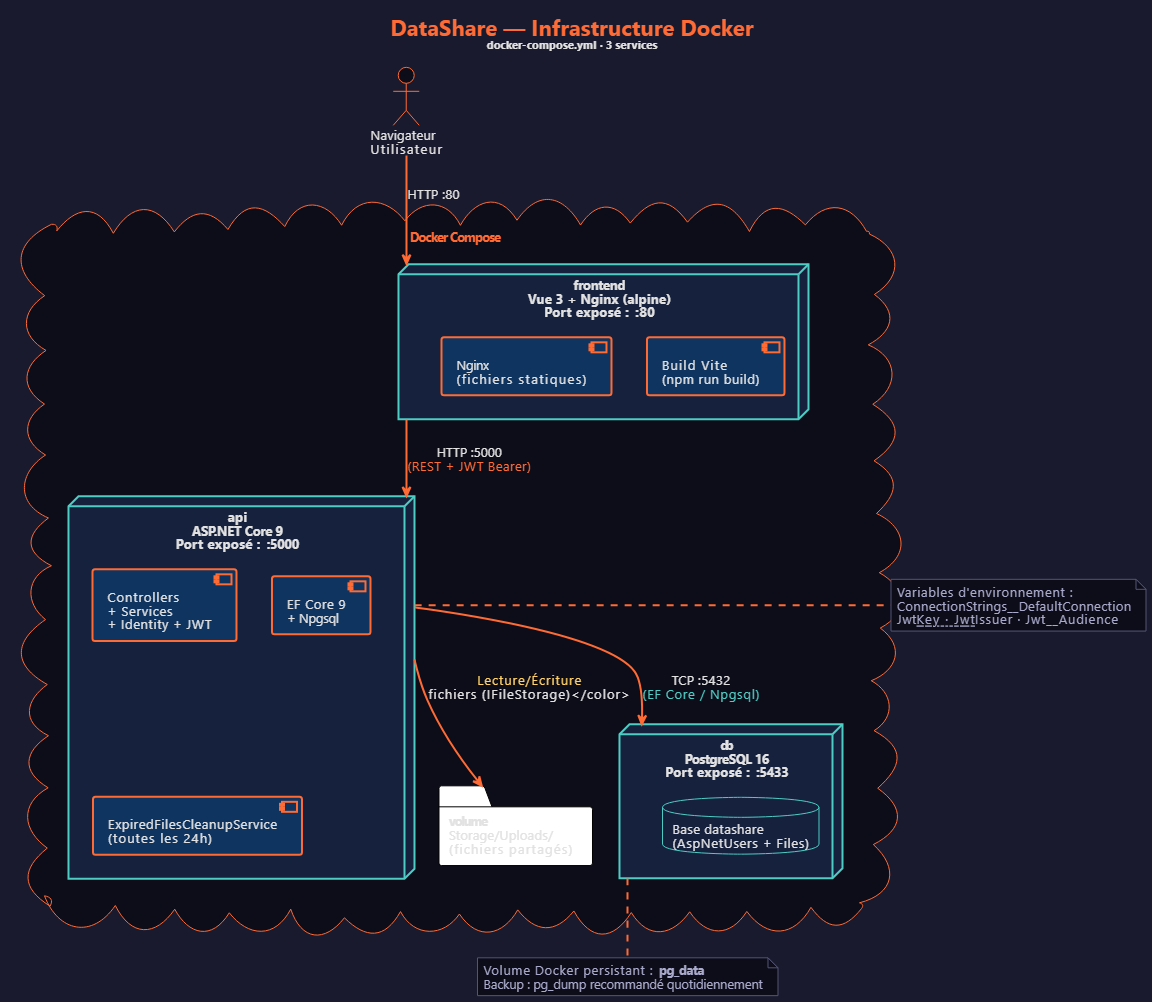
\includegraphics[width=\textwidth,keepaspectratio]{diagrams/infrastructure_docker.drawio.png}
  \caption{Infrastructure Docker --- trois services orchestr\'es par Docker Compose}
\end{figure}
\begin{itemize}[nosep]
  \item \textbf{db} --- PostgreSQL 16 sur le port 5433
  \item \textbf{api} --- API ASP.NET Core sur le port 5000
  \item \textbf{frontend} --- Vue 3 (Nginx) sur le port 80
\end{itemize}

\subsection{Variables d'environnement}

Le fichier \texttt{.env.example} fournit le template des variables \`a configurer :

\begin{longtable}{p{5cm} p{3cm} p{6cm}}
\toprule
\textbf{Variable} & \textbf{Exemple} & \textbf{Description} \\
\midrule
\endhead
\texttt{POSTGRES\_DB / \_USER / \_PASSWORD} & datashare / datashare / (secret) & Base, utilisateur et mot de passe PostgreSQL \\
\texttt{JWT\_KEY} & (32+ caract\`eres) & Cl\'e de signature JWT (l'API refuse de d\'emarrer sinon) \\
\texttt{JWT\_ISSUER / JWT\_AUDIENCE} & DataShareApi / DataShareClient & \'Emetteur et audience des tokens \\
\texttt{CORS\_ALLOWED\_ORIGINS} & http://localhost:5173 & Origine autoris\'ee (front hors nginx) \\
\texttt{VITE\_API\_URL} & /api & URL de l'API pour le build du front \\
\bottomrule
\end{longtable}

\textbf{Configuration compl\`ete (appsettings.json) :}

\begin{longtable}{p{6.5cm} p{7.5cm}}
\toprule
\textbf{Cl\'e} & \textbf{Description} \\
\midrule
\endhead
\texttt{ConnectionStrings:Default} & Cha\^ine de connexion PostgreSQL \\
\texttt{Jwt:Issuer} & \'Emetteur du token (d\'efaut : \texttt{DataShare}) \\
\texttt{Jwt:Audience} & Audience du token (d\'efaut : \texttt{DataShare}) \\
\texttt{Jwt:Key} & Cl\'e secr\`ete HMAC-SHA256 (min 32 caract\`eres) \\
\bottomrule
\end{longtable}

\texttt{docker-compose.yml} lit ces variables dans \texttt{.env} et les injecte dans la section \texttt{environment} du service \texttt{api} (\texttt{Section\_\_Cle} est lu par ASP.NET Core comme \texttt{Section:Cle}) :

\begin{lstlisting}
api:
  environment:
    ConnectionStrings__Default: "Host=db;Port=5432;Database=${POSTGRES_DB:-datashare};..."
    Jwt__Key: ${JWT_KEY:-change-me-in-production-secret-key-32chars}
    Jwt__Issuer: ${JWT_ISSUER:-DataShareApi}
    Jwt__Audience: ${JWT_AUDIENCE:-DataShareClient}
    Cors__AllowedOrigins__0: ${CORS_ALLOWED_ORIGINS:-http://localhost:5173}
\end{lstlisting}

%% ====================================================================
\section{Utilisation de l'IA dans le d\'eveloppement}
%% ====================================================================

\subsection{Posture adopt\'ee}

L'IA a \'et\'e utilis\'ee selon une approche \textbf{``assignation de t\^ache \`a un d\'eveloppeur junior''} pour la t\^ache principale (US08 --- Gestion des tags), puis en \textbf{bin\^omage ponctuel} pour le reste du projet.

\begin{longtable}{p{4cm} p{3.5cm} p{6.5cm}}
\toprule
\textbf{Phase} & \textbf{Outil} & \textbf{Usage} \\
\midrule
\endhead
D\'ebut de projet & ChatGPT & Aide g\'en\'erale, premi\`eres questions d'architecture \\
Questions complexes & Claude Opus (claude.ai) & Vision globale, d\'ecisions structurantes \\
D\'eveloppement & Claude Opus \& Sonnet (Cursor) & Opus pour le contexte complet du codebase, Sonnet pour les zones cibl\'ees \\
\bottomrule
\end{longtable}

L'\'evolution a \'et\'e naturelle : ChatGPT pour d\'emarrer, puis Claude Opus en ligne pour les r\'eflexions d'architecture, et enfin Cursor avec le codebase charg\'e pour le d\'eveloppement concret. Le passage \`a Cursor a permis \`a l'IA d'avoir le contexte projet complet, rendant les r\'eponses bien plus pertinentes.

\subsection{T\^ache principale : US08 --- Gestion des tags (frontend)}

\subsubsection{Contexte}

Le backend supportait d\'ej\`a les tags (\texttt{string[]} \`a l'upload, renvoy\'es dans les r\'eponses API). L'US08 consistait \`a impl\'ementer toute la partie frontend : champ de saisie de tags (chips) sur la page Upload, affichage des tags sur la page ``Mon espace'', et filtre local par tag (case-insensitive, contains).

\subsubsection{Fichiers modifi\'es par l'IA}

\begin{itemize}[nosep]
  \item \texttt{src/views/UploadView.vue} --- Champ de saisie de tags avec chips
  \item \texttt{src/views/MeView.vue} --- Affichage et filtrage par tags
  \item \texttt{src/styles/datashare.css} --- Styles des chips et du filtre
  \item (\texttt{src/api/files.ts} \'etait autoris\'e « si n\'ecessaire » : l'envoi des tags en \texttt{FormData} existait d\'ej\`a, aucune modification)
\end{itemize}

Le prompt complet est disponible dans le fichier \texttt{IA\_Instructions.txt} \`a la racine du projet. Tra\c{c}abilit\'e Git : commit \texttt{56f411d feat(ai): add tags UI and filtering} (code produit par l'IA) puis \texttt{a8c23fc fix(tags): show clear UI errors...} (revue humaine).

\subsection{Supervision et corrections humaines}

Apr\`es r\'eception du code g\'en\'er\'e par l'IA, les corrections suivantes ont \'et\'e apport\'ees manuellement :

\begin{longtable}{p{6cm} p{8cm}}
\toprule
\textbf{Probl\`eme d\'etect\'e} & \textbf{Correction} \\
\midrule
\endhead
Messages d'erreur UI absents pour tags invalides & Ajout de feedback visuel pour chaque cas d'erreur (vide, trop long, doublon) \\
Validation insuffisante c\^ot\'e UI & Renforcement des contr\^oles (trim, longueur max 24 caract\`eres, unicit\'e case-insensitive) \\
\bottomrule
\end{longtable}

\textbf{Processus de revue :}
\begin{enumerate}[nosep]
  \item Lecture compl\`ete du diff g\'en\'er\'e par l'IA.
  \item Test manuel des cas limites (tag vide, tag > 24 caract\`eres, doublon exact, doublon casse diff\'erente).
  \item Identification des lacunes UX (aucun message d'erreur pour l'utilisateur).
  \item Correction et commit s\'epar\'e pour tra\c{c}abilit\'e.
\end{enumerate}

\textbf{Points de vigilance v\'erifi\'es :} le back reste l'autorit\'e (normalisation et d\'eduplication des tags aussi c\^ot\'e API, 20 tags max) ; aucune nouvelle d\'ependance ; styles ajout\'es dans \texttt{datashare.css} avec le pr\'efixe \texttt{ds-} existant ; logique isol\'ee dans \texttt{addTag} / \texttt{removeTag} ; conformit\'e \`a la charte Figma.

\subsection{Autres usages de l'IA}

\begin{longtable}{p{4cm} p{10cm}}
\toprule
\textbf{Usage} & \textbf{D\'etail} \\
\midrule
\endhead
Audit de code & Revue de s\'ecurit\'e, d\'etection de d\'ependances inutiles, v\'erification de coh\'erence \\
Debugging & R\'esolution d'erreurs CORS, JWT, configuration Docker \\
Architecture & Conseils sur l'organisation Services/Models/Controllers \\
Recherche technique & Bonnes pratiques .NET, Vue 3, PostgreSQL --- remplace efficacement Google/Stack Overflow \\
Documentation & Assistance r\'edaction des fichiers \texttt{.md} techniques \\
Revue finale avant soutenance (09/2026) & Audit de coh\'erence code $\leftrightarrow$ documentation (OpenAPI p\'erim\'e, \texttt{SECURITY.md} d\'ecrivant des m\'ecanismes absents du code), propositions de tests de s\'ecurit\'e et de logs structur\'es, relecture du support ; chaque proposition relue, ex\'ecut\'ee (\texttt{dotnet test}, \texttt{npm run build}) et valid\'ee avant commit \\
\bottomrule
\end{longtable}

\subsection{Apports et limites constat\'es}

\subsubsection{Apports}

\begin{itemize}[nosep]
  \item \textbf{Gain de temps :} US08 compl\`ete ($\sim$200 lignes, 4 fichiers) produite en $\sim$15 minutes contre $\sim$2 heures estim\'ees manuellement.
  \item \textbf{Audit efficace :} d\'etection rapide de probl\`emes de s\'ecurit\'e et de d\'ependances inutiles.
  \item \textbf{Recherche contextuelle :} r\'eponses adapt\'ees au projet, pas de r\'eponses g\'en\'eriques.
  \item \textbf{Coh\'erence :} code g\'en\'er\'e respectant le style existant du projet.
\end{itemize}

\subsubsection{Limites}

\begin{itemize}[nosep]
  \item \textbf{UX n\'eglig\'ee :} l'IA n'a pas pens\'e aux messages d'erreur utilisateur.
  \item \textbf{Pas de tests spontan\'es :} aucun test propos\'e pour le code g\'en\'er\'e.
  \item \textbf{Supervision indispensable :} sans revue humaine, les cas limites auraient \'et\'e livr\'es sans feedback utilisateur.
\end{itemize}

\subsection{Conclusion sur l'utilisation de l'IA}

L'IA s'est r\'ev\'el\'ee efficace comme outil de productivit\'e \`a tous les niveaux du projet. L'approche ``junior supervis\'e'' pour l'US08 a bien fonctionn\'e, et l'usage en bin\^omage pour le reste (audit, debug, recherche) a significativement acc\'el\'er\'e le d\'eveloppement. La supervision humaine reste indispensable pour la qualit\'e UX et la couverture de tests.

\end{document}
